% This is samplepaper.tex, a sample chapter demonstrating the
% LLNCS macro package for Springer Computer Science proceedings;
% Version 2.20 of 2017/10/04
%
\documentclass[runningheads]{llncs}
%
\usepackage{graphicx}
\usepackage{longtable}
\graphicspath{ {./images/} }
% Used for displaying a sample figure. If possible, figure files should
% be included in EPS format.
%
% If you use the hyperref package, please uncomment the following line
% to display URLs in blue roman font according to Springer's eBook style:
% \renewcommand\UrlFont{\color{blue}\rmfamily}

\begin{document}
%
\title{Linear Algebra Assignment II}
%
%\titlerunning{Abbreviated paper title}
% If the paper title is too long for the running head, you can set
% an abbreviated paper title here
%
\author{Akash Panda {+91-9654659108}}
%
\authorrunning{Linear Algebra Assignment - II}
% First names are abbreviated in the running head.
% If there are more than two authors, 'et al.' is used.
%
\institute{Indian Institute of Science Bangalore, India\\
\email{akashpanda@iisc.ac.in}\\
\url{http://akashiisc.github.io}}
%
\maketitle              % typeset the header of the contribution
%
%
%
%
\section{Problem - I}
\subsection{Task I}
For the given dataset, the graph plotted is shown below.\\
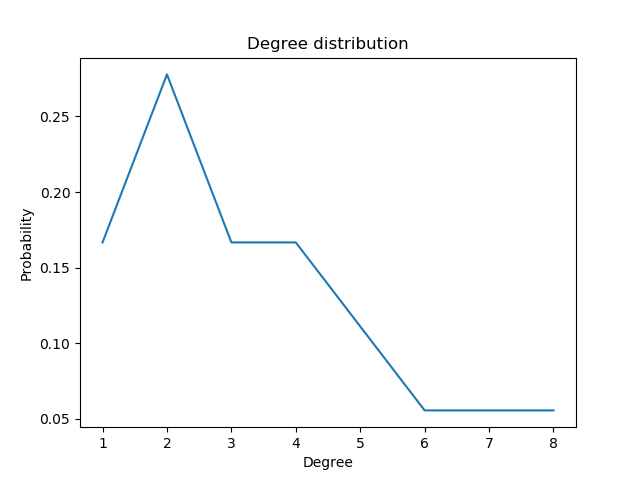
\includegraphics[scale=0.5]{problem_1_task_1} \\
We can see this distribution somewhat similar to inverse gaussian distribution.
\subsection{Task V}
For the test data given, 
Min eigen value was found to be : \[-1.3813844561213333e^{-16}\]  (which is close to zero)\\
and Eigen vector corresponding to the minimum eigen value is obtained as 
Transpose of \
[0.23570226039551526 0.2357022603955154 0.2357022603955153\\
0.23570226039551526 0.2357022603955154 0.23570226039551562,\\
0.23570226039551528 0.2357022603955153 0.23570226039551626,\\
0.23570226039551626 0.23570226039551626 0.23570226039551642,\\
0.23570226039551634 0.23570226039551628 0.23570226039551628,\\
0.23570226039551628 0.2357022603955163 0.23570226039551614] , which is a scaled version of all 1's


\subsection{Task VI}
For the given test data, the following coloured plot is found \\
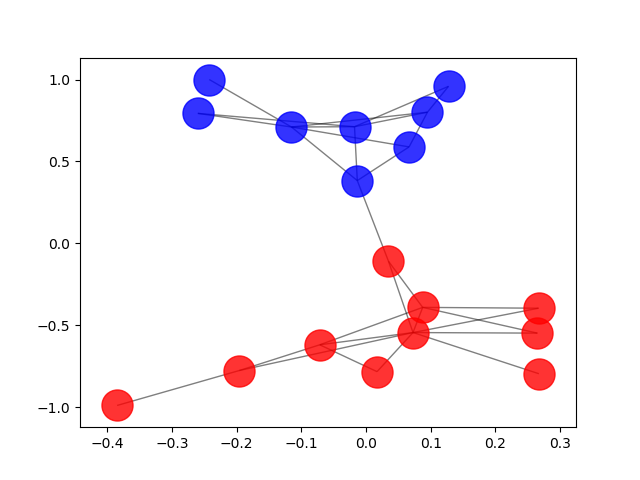
\includegraphics[scale=0.5]{problem_1_task_6} \\
It is observed that, the points are being clustered into two different groups.
The graph is being divided by the cut edge. The edge joining the two clusters is a cut edge (i.e. if it is removed the graph will have 2 connected components.)

\subsection{Bonus I}
For the given test data, the following coloured plot is found using \textbf{numpy} \\
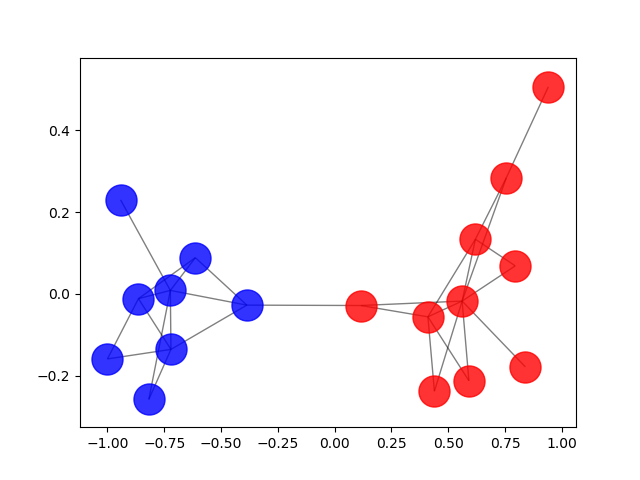
\includegraphics[scale=0.5]{problem_1_bonus_1} \\
No difference in clustering is observed. 

\subsection{Bonus II}
If we are asked to divide into more than 2 clusters, then we can do so by taking more than 1 eigen vectors. For example, we can take the eigen vectors corresponding to second smallest and third smallest eigen value. Now we can divide the nodes into 4 clusters (according to sign of the corresponding entries of eigen vector elements)
[i.e. + + , + - , - - , - +]
In this way,  if we take m eigen vectors, we can cluster the nodes into $2^n$ clusters.

\subsection{Bonus III}
The below plot is observed if we take the second largest eigen vector instead of second smallest. \\
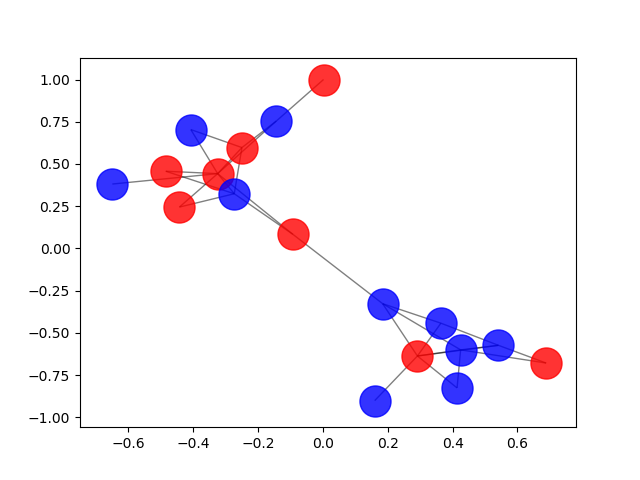
\includegraphics[scale=0.5]{problem_1_bonus_3} \\
My observation is that the clustering is not perfect as it was with the second smallest eigen vector. 

\subsection{Bonus IV}
The central edge of the graph is the edge that has one node in each of the clusters.(as observed)
\section{Problem - II}
\subsection{Task II}
\begin{longtable}{| p{.20\textwidth} | p{.20\textwidth} | p{.20\textwidth} |} 
\hline
M & K & Accuracy\\
\hline
1 & 1 & 0.2365 \\
1 & 3 & 0.2535 \\
2 & 1 & 0.396 \\
2 & 3 & 0.405 \\
3 & 1 & 0.465 \\
3 & 3 & 0.481 \\
4 & 1 & 0.573 \\
4 & 3 & 0.5945 \\
1 & 5 & 0.267 \\
1 & 10 & 0.27 \\
1 & 15 & 0.273 \\
2 & 5 & 0.4135 \\
2 & 10 & 0.4325 \\
2 & 15 & 0.438 \\
3 & 5 & 0.4975 \\
3 & 10 & 0.515 \\
3 & 15 & 0.512 \\
4 & 5 & 0.607 \\
4 & 10 & 0.6235 \\
4 & 15 & 0.6315 \\
5 & 1 & 0.707 \\
5 & 3 & 0.7185 \\
5 & 5 & 0.7345 \\
5 & 10 & 0.745 \\
5 & 15 & 0.7455 \\
5 & 20 & 0.7435 \\
6 & 1 & 0.7945 \\
6 & 3 & 0.8275 \\
6 & 5 & 0.835 \\
6 & 10 & 0.8375 \\
6 & 15 & 0.8335 \\
6 & 20 & 0.843 \\
7 & 1 & 0.8365 \\
7 & 3 & 0.8545 \\
7 & 5 & 0.865 \\
7 & 10 & 0.8615 \\
7 & 15 & 0.8625 \\
7 & 20 & 0.857 \\
8 & 1 & 0.881 \\
8 & 3 & 0.8845 \\
8 & 5 & 0.8945 \\
8 & 10 & 0.887 \\
8 & 15 & 0.8925 \\
8 & 20 & 0.8905 \\
9 & 1 & 0.891 \\
9 & 3 & 0.8965 \\
9 & 5 & 0.902 \\
9 & 10 & 0.9005 \\
9 & 15 & 0.8965 \\
9 & 20 & 0.8875 \\
10 & 1 & 0.9055 \\
10 & 3 & 0.91 \\
10 & 5 & 0.9195 \\
10 & 10 & 0.9145 \\
10 & 15 & 0.9145 \\
10 & 20 & 0.904 \\
11 & 1 & 0.9135 \\
11 & 3 & 0.924 \\
11 & 5 & 0.9315 \\
11 & 10 & 0.9245 \\
11 & 15 & 0.9215 \\
11 & 20 & 0.9175 \\
12 & 1 & 0.921 \\
12 & 3 & 0.9335 \\
12 & 5 & 0.9355 \\
12 & 10 & 0.926 \\
12 & 15 & 0.925 \\
12 & 20 & 0.9215 \\
13 & 1 & 0.9305 \\
13 & 3 & 0.9385 \\
13 & 5 & 0.9425 \\
13 & 10 & 0.9325 \\
13 & 15 & 0.931 \\
13 & 20 & 0.927 \\
14 & 1 & 0.9385 \\
14 & 3 & 0.9495 \\
14 & 5 & 0.9485 \\
14 & 10 & 0.9335 \\
14 & 15 & 0.942 \\
14 & 20 & 0.932 \\
15 & 1 & 0.9395 \\
15 & 3 & 0.949 \\
15 & 5 & 0.947 \\
15 & 10 & 0.9355 \\
15 & 15 & 0.9365 \\
15 & 20 & 0.9325 \\
16 & 1 & 0.9515 \\
16 & 3 & 0.959 \\
16 & 5 & 0.959 \\
16 & 10 & 0.946 \\
16 & 15 & 0.944 \\
16 & 20 & 0.937 \\
17 & 1 & 0.9545 \\
17 & 3 & 0.96 \\
17 & 5 & 0.958 \\
17 & 10 & 0.9445 \\
17 & 15 & 0.949 \\
17 & 20 & 0.9415 \\
18 & 1 & 0.955 \\
18 & 3 & 0.959 \\
18 & 5 & 0.9565 \\
18 & 10 & 0.951 \\
18 & 15 & 0.95 \\
18 & 20 & 0.942 \\
19 & 1 & 0.9585 \\
19 & 3 & 0.9625 \\
19 & 5 & 0.959 \\
19 & 10 & 0.952 \\
19 & 15 & 0.95 \\
19 & 20 & 0.9455 \\
20 & 1 & 0.9585 \\
20 & 3 & 0.9645 \\
20 & 5 & 0.9635 \\
20 & 10 & 0.956 \\
20 & 15 & 0.9555 \\
20 & 20 & 0.945 \\
21 & 1 & 0.9565 \\
21 & 3 & 0.9635 \\
21 & 5 & 0.9625 \\
21 & 10 & 0.9555 \\
21 & 15 & 0.955 \\
21 & 20 & 0.95 \\
22 & 1 & 0.959 \\
22 & 3 & 0.964 \\
22 & 5 & 0.963 \\
22 & 10 & 0.9595 \\
22 & 15 & 0.9545 \\
22 & 20 & 0.947 \\
23 & 1 & 0.9605 \\
23 & 3 & 0.966 \\
23 & 5 & 0.962 \\
23 & 10 & 0.955 \\
23 & 15 & 0.9575 \\
23 & 20 & 0.95 \\
24 & 1 & 0.963 \\
24 & 3 & 0.966 \\
24 & 5 & 0.968 \\
24 & 10 & 0.9615 \\
24 & 15 & 0.9605 \\
24 & 20 & 0.951 \\
25 & 1 & 0.9655 \\
25 & 3 & 0.9675 \\
25 & 5 & 0.9685 \\
25 & 10 & 0.9595 \\
25 & 15 & 0.9555 \\
25 & 20 & 0.9545 \\
26 & 1 & 0.9655 \\
26 & 3 & 0.9675 \\
26 & 5 & 0.9655 \\
26 & 10 & 0.9585 \\
26 & 15 & 0.9595 \\
26 & 20 & 0.952 \\
27 & 1 & 0.968 \\
27 & 3 & 0.9665 \\
27 & 5 & 0.966 \\
27 & 10 & 0.965 \\
27 & 15 & 0.9615 \\
27 & 20 & 0.9555 \\
28 & 1 & 0.9695 \\
28 & 3 & 0.9655 \\
28 & 5 & 0.9665 \\
28 & 10 & 0.964 \\
28 & 15 & 0.9635 \\
28 & 20 & 0.953 \\
29 & 1 & 0.9695 \\
29 & 3 & 0.9665 \\
29 & 5 & 0.9685 \\
29 & 10 & 0.9625 \\
29 & 15 & 0.9595 \\
29 & 20 & 0.9505 \\
\hline
\end{longtable}

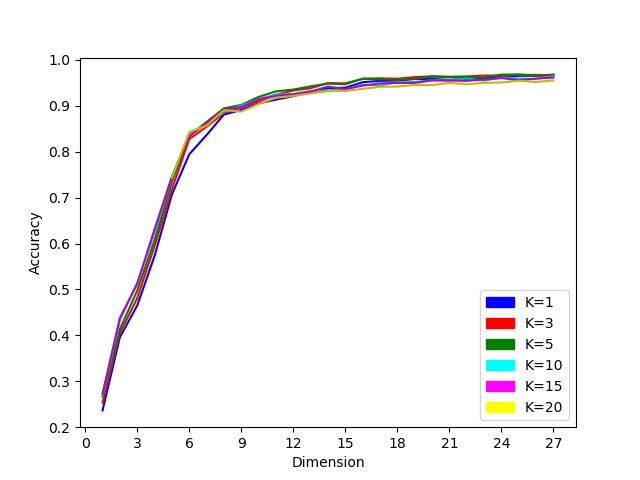
\includegraphics[scale=0.8]{k-n-accuracy}
The above graph represents the data that is reported in above table.\\
By observing the above accuracy plots, I choose \textbf{M=20} and \textbf{K=3} for the model.

\subsection{Bonus I}
The vectors, when projected to 2D space resulted in the below figure:\\
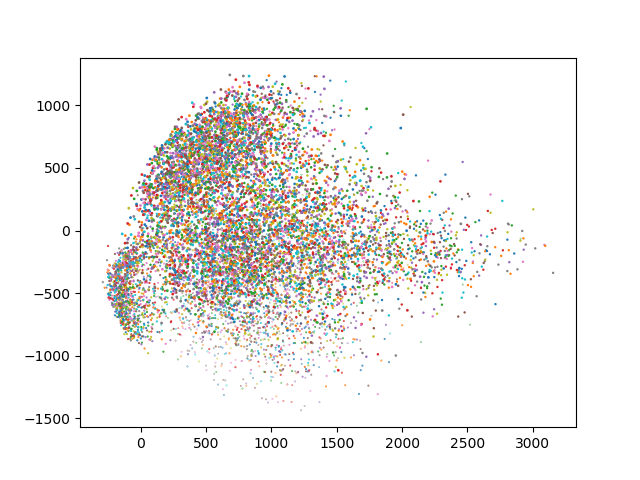
\includegraphics[scale=0.8]{problem_2_bonus_1}\\
No observation could be made from above figure.

\subsection{Bonus II}

%
% ---- Bibliography ----
%
% BibTeX users should specify bibliography style 'splncs04'.
% References will then be sorted and formatted in the correct style.
%
% \bibliographystyle{splncs04}
% \bibliography{mybibliography}
%
\begin{thebibliography}{1}
\bibitem{ref_proc1}
https://stackoverflow.com/questions/16569613/how-does-numpy-linalg-inv-calculate-the-inverse-of-an-orthogonal-matrix
\end{thebibliography}
\end{document}
